\documentclass[epsfig]{article}
\usepackage{epsfig}
\usepackage{amsmath}
\usepackage{verbatim}
\usepackage{booktabs}
\usepackage{subfig}
\usepackage{graphicx}
\usepackage[english]{babel}
\usepackage{float}
\textwidth 6.7in
\oddsidemargin -0.1in
\textheight 8.50in
\topmargin -0.55in
\renewcommand{\textfraction}{0.25}
\renewcommand{\floatpagefraction}{0.7}
\markboth{}{\sl E. Mer\'enyi \hfil COMP / ELEC / STAT 502 \hfil Homework 4 }
\pagestyle{myheadings}
\def\bpar{\vskip26pt}
\def\npar{\vskip13pt}
\def\spar{\vskip10pt}
\begin{document}
\parindent=0pt
\null



{\bf 
\npar
Problem 2
\bpar
}


\begin{table}[htbp] 
\center
\caption{Parameters of Training BP Network to perform the equalization of the communication channel}
  \label{tab:NP}
  %\scalebox{0.9}{ % You can scale the size of the table by changing this number
   \scalebox{1.0}{
   \begin{tabular}{p{4cm} p{.05cm} p{8cm}}
\toprule
  \multicolumn{3}{l}{\bf Network parameters} \\
\bottomrule \noalign{\smallskip}
  Topology & & $(1 + 1_{Bias})$ --- $(10 + 1_{Bias})$ (otherwise notified) --- $1$ \\
  Transfer function & & tanh with slope of 1 \\
\toprule
  \multicolumn{3}{l}{\bf Learning parameters} \\
\bottomrule \noalign{\smallskip}
  Initial weights & & drawn from U[-0.1, 0.1] \\
  Learning rate ($\alpha$) & & 0.01, otherwise notified\\
  Momentum & & 0.9\\
  Epoch size ($Epoch$)& &  20\\
  Stopping criteria & &  error ($Err_{RMSD}$) $<$ 0.01 or learn steps =60,000\\
  Monitoring frequency of error measure & &  Every 1000 learn steps\\
  Error measure($Err_{RMSD}$) & &  Square root of the sum of $(D-y)^2$ that averaged over all training or testing samples (see formula (1) in problem 2)\\\toprule
 \multicolumn{3}{l}{\bf Input / output data, representation, scaling} \\
\bottomrule \noalign{\smallskip}
  \ Training samples ($S{(n)}$)& & $2sin({2\pi n \over 20}) $, $n$=1,2,3.. Twenty training samples in total\\ 
    \ Test sample set 1 ($s_1{(n)}$)& & 20 numbers in $0.8sin({2\pi n \over 10}) + 0.25cos({2\pi n \over 25})$\\
    \ Test sample set 2 ($s_2{(n)}$)& & 50 random numbers drawn from a zero mean, unit variance normal distribution\\
  Scaling of inputs & & Map [global min, global max] to [-1,1]\\
  Scaling of training and test1 outputs & &  Map [global min, global max] to [-1,1] \\
  Scaling of test2 inputs & &  Map [local min, local max] to [-1,1] \\
 \bottomrule \noalign{\smallskip}
 
  \end{tabular}
   } % end scalebox
\end{table}


For all the output verses desired output plots, we used z(nT) as input(x axis), and $\hat{s}$(nT), s(nT) as output(y axis). 

\clearpage
{\bf 
\npar
2.1) Training
\bpar
}

For the first several steps, the MSE dropped dramatically (from 0.8 to less than 0.1, for example) and it makes it hard to view the history after that. Therefore, we start our history from step 1000 (50*20, where 20 is the epoch size).  

The MSE history is shown below:

\begin{figure}[!htb] 
\centering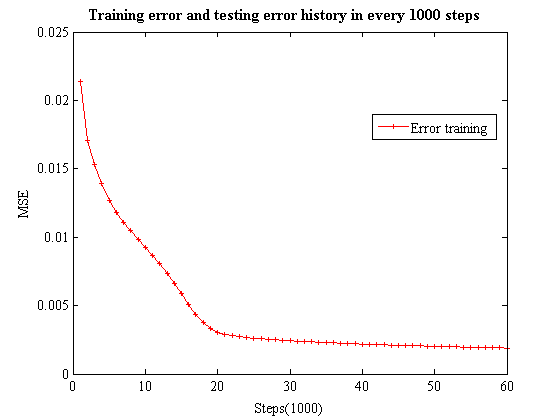
\includegraphics[width=4in]{MSEhistory_1.png} 
\end{figure} 

The training output versus desired output is shown as figure below.

\begin{figure}[!htb] 
\centering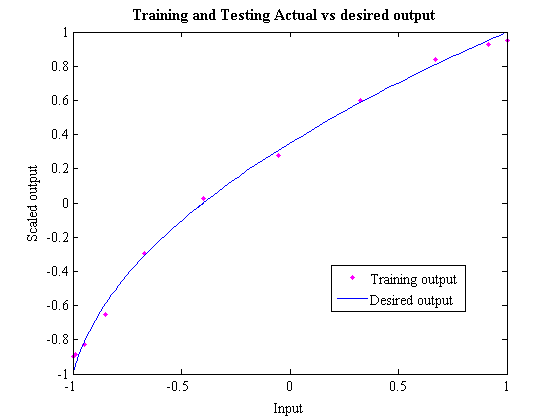
\includegraphics[width=4in]{TrainvsDesire_1.png} 
\end{figure} 

\clearpage

{\bf 
\npar
2.1.1) Different hidden PE number
\bpar
}

We first tried to use different number of hidden PE. By comparing the history, increasing the number of hidden PE did not significantly change the reduction of MSE, except for $\#$PE=1. For $\#$PE=1, it took longer time to reduce the MSE. The final error rate for $\#$PE=1, $\#$PE=5, $\#$PE=10, $\#$PE=80 are  0.0019, 0.0020, 0.0019, 0.0029. We noticed that the final MSE varied during repeating the training, so these values can only show that their final result were qualitatively the same.

In this case, the final output of training were almost overlapped to $\#$PE=10, so the training data vs desired data for each condition is not shown here.

\begin{figure}[!htb] 
\centering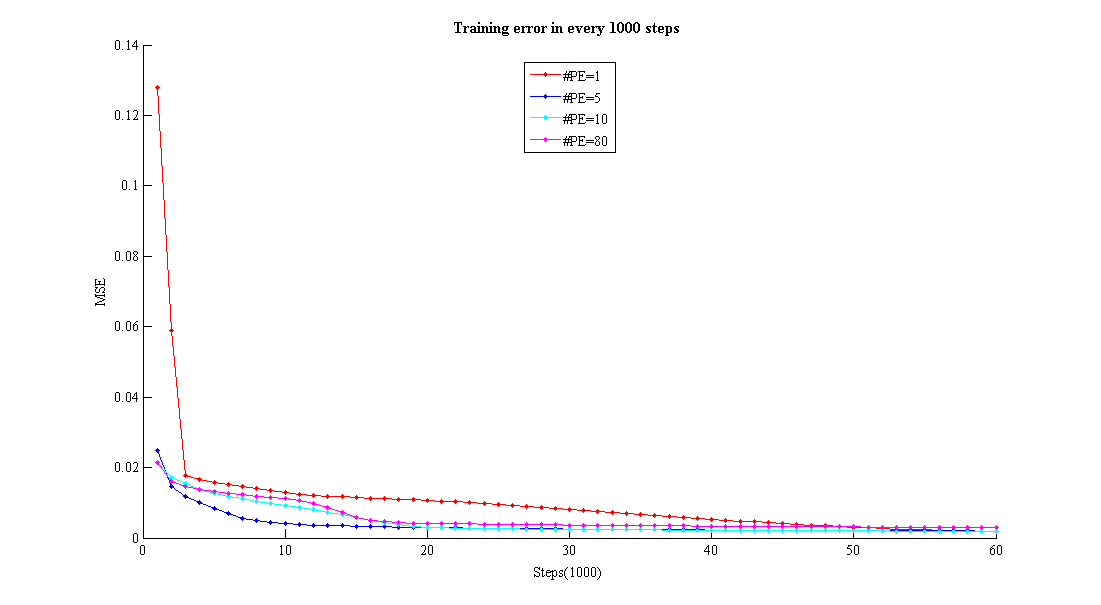
\includegraphics[width=6.5in]{errPE.png} 
\end{figure} 

\clearpage

{\bf 
\npar
2.1.2) Different learning rate
\bpar
}

We used 0.01, 0.015 and 0.05 as learning rate. Interestingly, we found two patterns when learning rate is equal to 0.05. As shown below, the large learning rate can help the neuron network get to a small MSE much faster than the others and meet the criteria of stopping. The learning met the MSE less than or equal to 0.0015 criteria at 27000 step.

\begin{figure}[!htb] 
\centering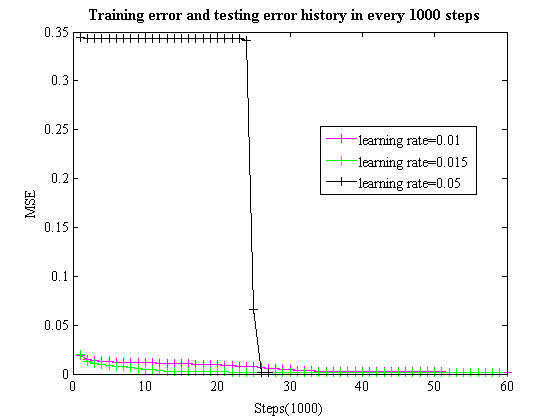
\includegraphics[width=4.5in]{lr_err1.png} 
\end{figure} 

Because of the limitation of training input (n need to be integers), the training data are kind of overlapping.

\begin{figure}[!htb] 
\centering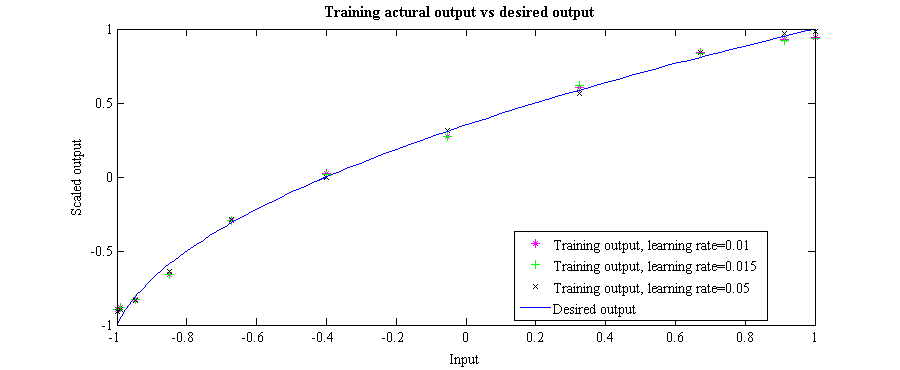
\includegraphics[width=6.5in]{lr_out1.png} 
\end{figure} 




\clearpage

However, in some other cases, using 0.05 as learning rate cannot converge the MSE, which is shown as figure below:

\begin{figure}[!htb] 
\centering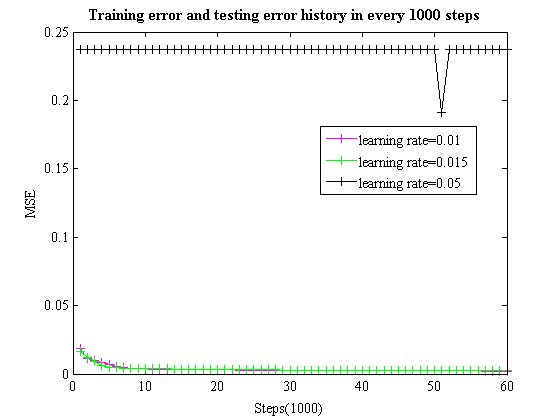
\includegraphics[width=4.5in]{lr_err2.png} 
\end{figure} 

And the learning failed(see the small black x at the top and the bottom). 

\begin{figure}[!htb] 
\centering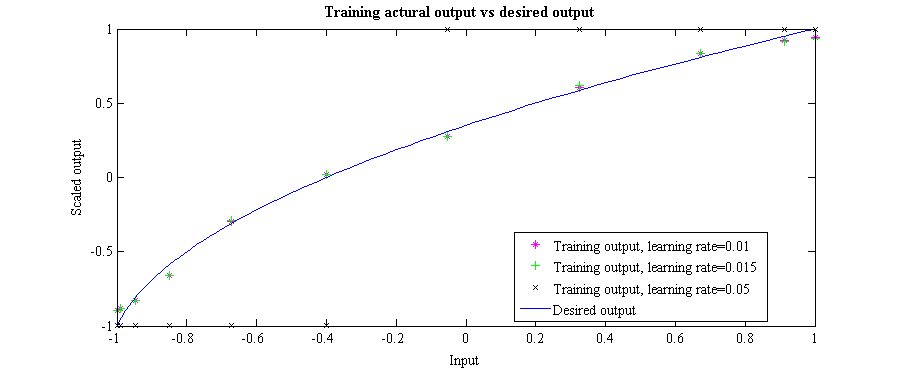
\includegraphics[width=6.5in]{lr_out2.png} 
\end{figure} 

\clearpage

{\bf 
\npar
2.2.1) Test the memory using $s_1{(n)}0.8sin({2\pi n \over 10}) + 0.25cos({2\pi n \over 25})$

\bpar
}

Test group 1: $s_1{(n)}0.8sin({2\pi n \over 10}) + 0.25cos({2\pi n \over 25})$

The MSE history is shown as below. We can see that the testing error is higher than training error.

\begin{figure}[!htb] 
\centering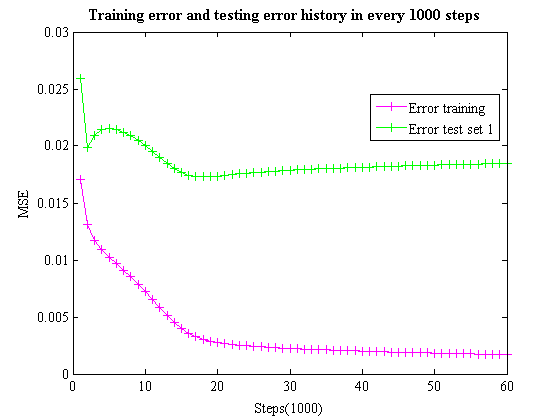
\includegraphics[width=4.5in]{err_test1.png} 
\end{figure} 

The training, testing output versus desired output is shown as figure below, where the final MSE is 0.0185 for testing, 0.0026 for training.

\begin{figure}[!htb] 
\centering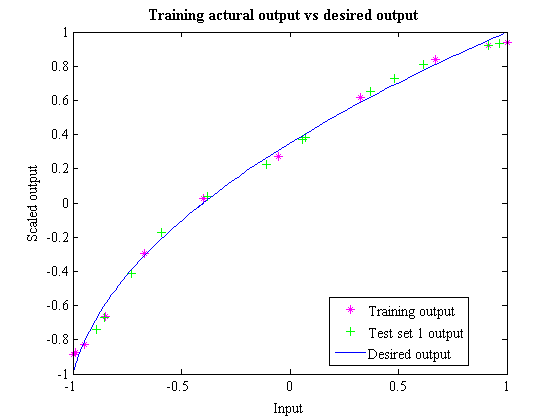
\includegraphics[width=4.5in]{output_test1.png} 
\end{figure} 

We also checked the performance after scaling back. The range of network input was limited around [-1,1], so they are stacking in the middle of the curve, and the data is shown below:

\begin{figure}[!htb] 
\centering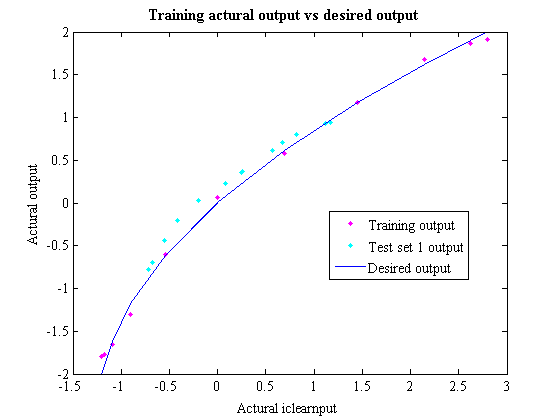
\includegraphics[width=4.5in]{output_test1_rs.png} 
\end{figure} 


\clearpage

{\bf 
\npar
2.2.1) Test the memory using test group 2

\bpar
}


Test group 2: $s_2{(n)}$), 50 random numbers drawn from a zero mean, unit variance normal distribution.


The MSE history is shown as below.  The final MSE for testing group is 0.0028, for training group is 0.0024.

\begin{figure}[!htb] 
\centering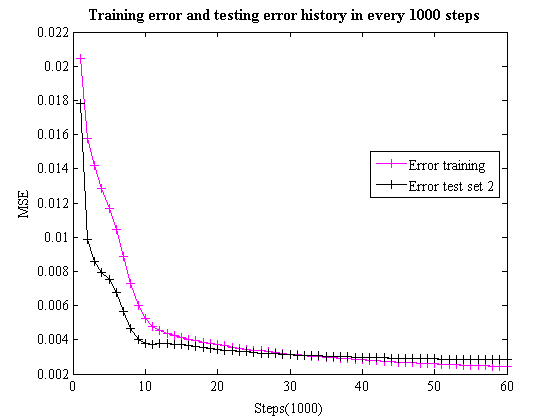
\includegraphics[width=4.5in]{err_test2.png} 
\end{figure} 

The training, testing output versus desired output is shown as figure below:

\begin{figure}[!htb] 
\centering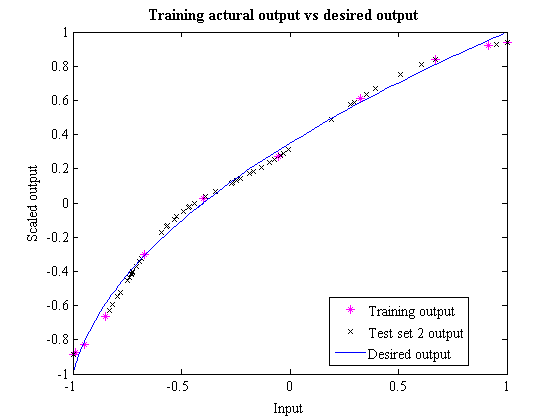
\includegraphics[width=4.5in]{output_test2.png} 
\end{figure} 

\end{document}